\documentclass[12pt]{article}
\usepackage{enumitem}
\usepackage{titling}
\usepackage{graphicx}
\graphicspath{{img/}}
\usepackage{subfig}
\newcommand{\subtitle}[1]{%
	\posttitle{%
		\par\end{center}
	\begin{center}\large#1\end{center}}%
}

\title{\bf{Server Cluster Load Balancing}}
\subtitle{https://github.com/nikhilsidhu/server-network-simulation}
\author{Nikhil Sidhu}

\begin{document}
\maketitle

\section{Intro}
	\par The motivation for this project comes from the desire to optimize resource utilization in server networks. Although it is possible to make more powerful servers, at the end of the day this becomes expensive and has diminishing returns. Load balancing refers to the distribution of traffic within a network, in an attempt to improve server availability and efficiency of processing. 
	
	The set up for this project involves using 5 slow and 3 fast servers handling requests (fig.1), along with two load balancing algorithms that determine where the network traffic flows. The first algorithm is simple, directing requests to the server node with the shortest queue. The more advanced algorithm prefers to send traffic to the faster servers as much as possible to maximize efficiency. 
	
	\begin{figure}[h]
		\centering
		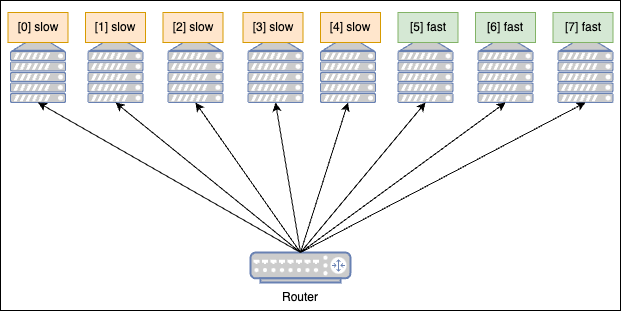
\includegraphics[width=\textwidth]{server-network}
		\caption{Layout of the server network}
	\end{figure}

\section{Libraries}
	\begin{description}
		\item [Ciw] - event simulation for open queuing networks, packet-switched networks are of this kind.
		\item [numpy] - used for calculations
		\item [matplotlib] - used for creating graphs
	\end{description}

\section{Instructions}
	\par Simply run the simulation with 'python3 Network.py'. Matplotlib will open the graphs for each run at the end of simulation, these can be closed to end the program.

\section{Results}
	\par The results were as expected, the simple load balancer performed worse than the more advanced algorithm, that preferentially selects faster servers, after convergence (fig. 2).

	\begin{figure}[h]
	\centering
	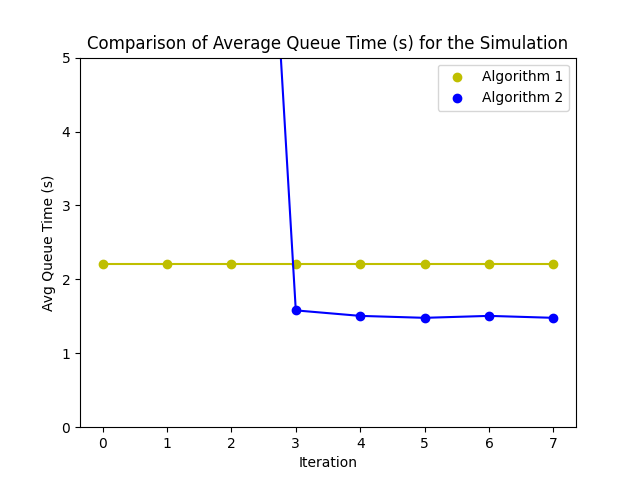
\includegraphics[width=\textwidth]{queue}
	\caption{Average queue time in each iteration}
	\end{figure}

	The server utilization for the simple algorithm is high for all servers (fig.3). When the second algorithm is executed, we see that the slow servers aren't even used in the first block of time that is simulated (fig.4), as they aren't at full load. In the second iteration, the slow servers begin to be used at a slow rate (fig.5). By the last iteration, the algorithm has reached convergence and the numbers stabilize (fig.6).
	
	\begin{figure}[h]
		\centering
		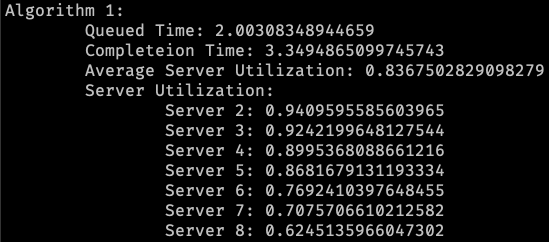
\includegraphics[width=\textwidth]{alg1}
		\caption{Average server utilization for the simple algorithm}
	\end{figure}

	\begin{figure}[h]
		\centering
		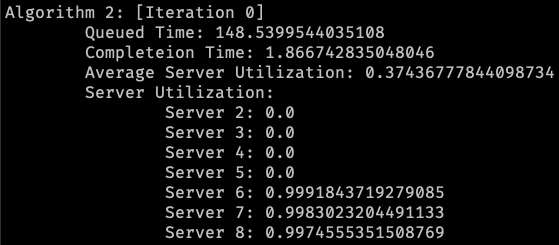
\includegraphics[width=\textwidth]{iter0}
		\caption{Server utilization in algorithm 2 iteration 0}
	\end{figure}

	\begin{figure}[h]
		\centering
		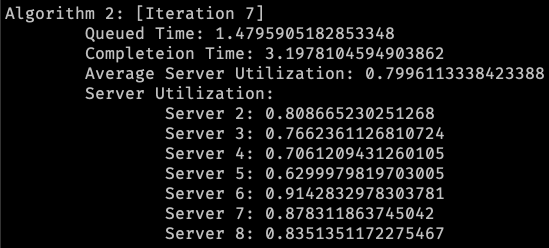
\includegraphics[width=\textwidth]{iter7}
		\caption{Server utilization in algorithm 2 iteration 7}
	\end{figure}

\section{Discussion}
	\par It would be interesting to experiment with larger server clusters and also having servers shut down randomly to simulate failure. There are much more advanced algorithms for load balancing and implementing those in such a setting could be a useful tool when paired with differently structured networks. 

\section{Papers Referenced}
	\begin{description}
		\item https://sites.pitt.edu/~dtipper/2130/2130\_Slides5.pdf
		\item https://ieeexplore-ieee-org.uml.idm.oclc.org/abstract/document/4403185
		\item https://ieeexplore-ieee-org.uml.idm.oclc.org/abstract/document/8368317
	\end{description}

\end{document}